\documentclass{article}

\usepackage{graphicx}
\usepackage{caption}
\usepackage{subcaption}

\usepackage{sidecap}

\begin{document}


\section{something}

\begin{figure}[htb]
\parbox{.3\linewidth}{
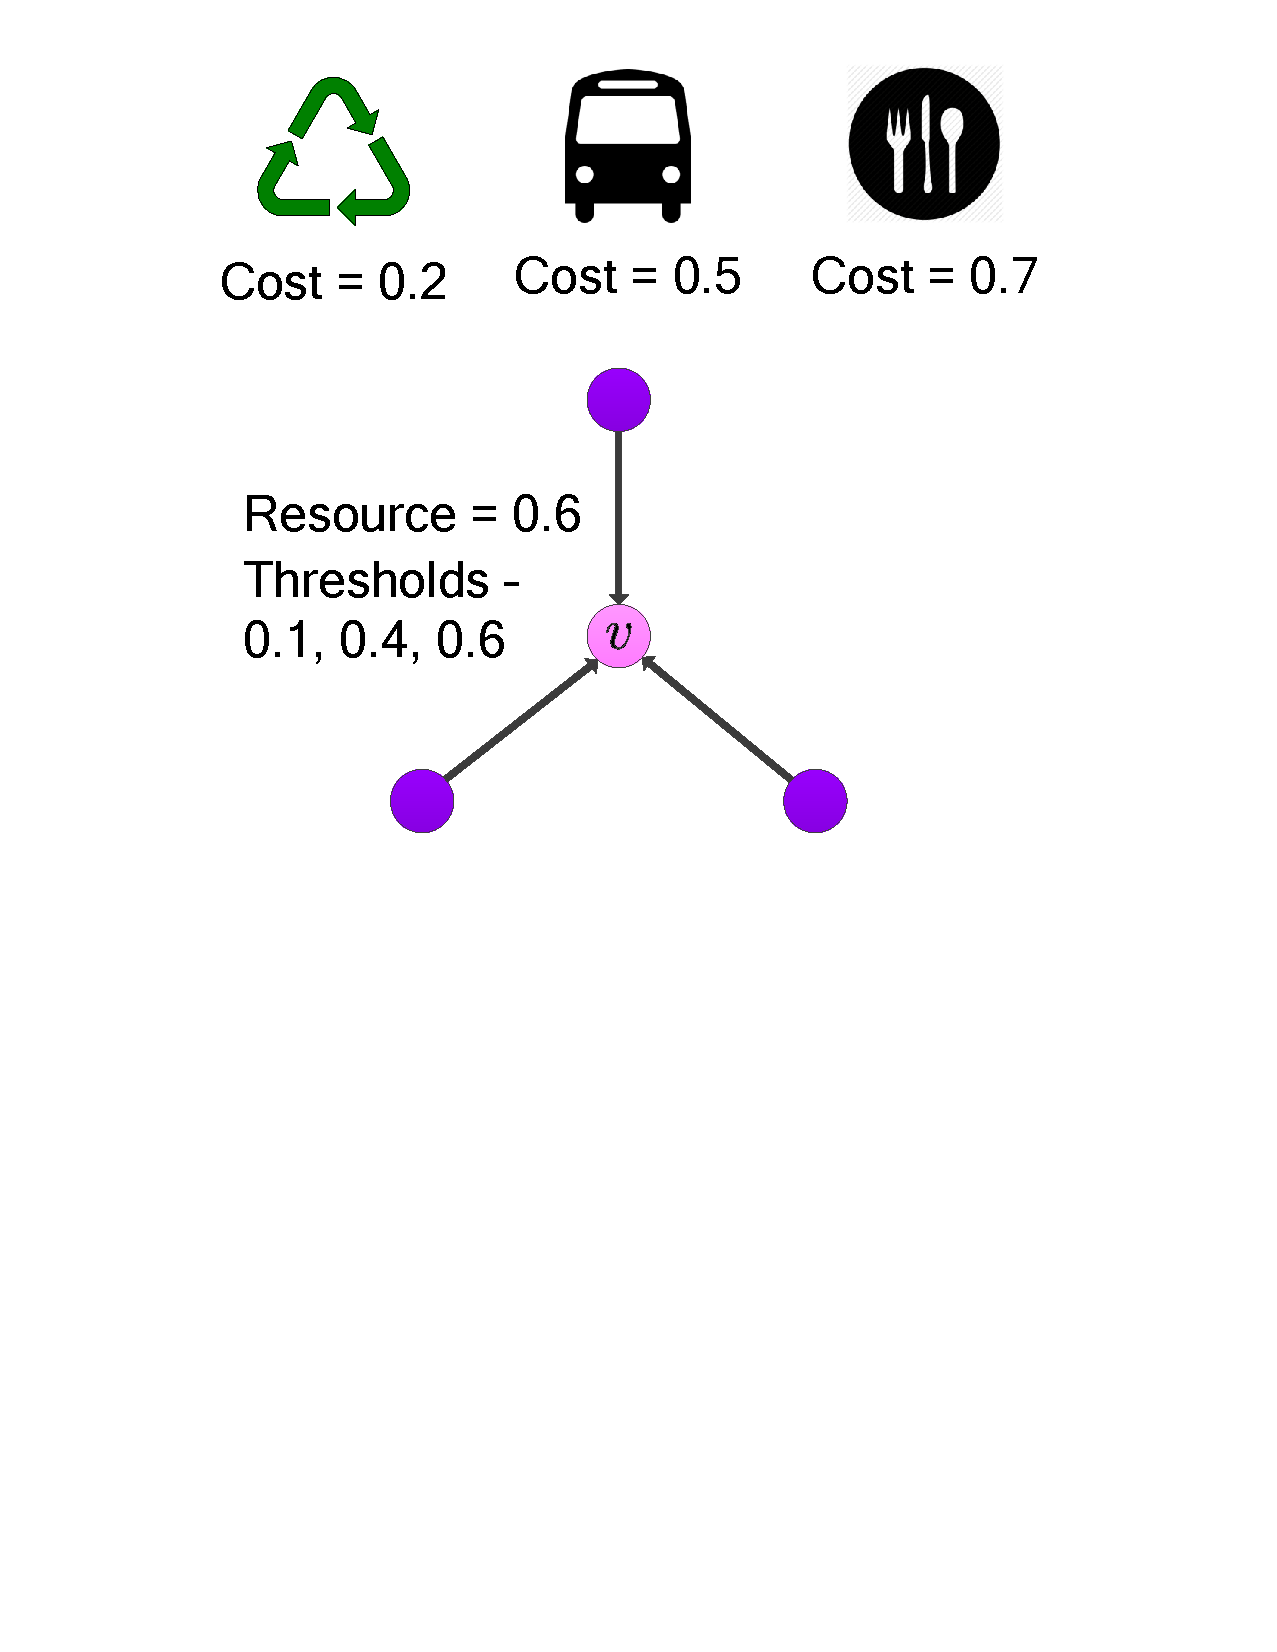
\includegraphics[viewport=1.25in 4in 7in 11in, width=\linewidth]{figs/timeline-1a}}%
\hspace{.2\linewidth}%
\parbox[][][t]{.3\linewidth}{%
\subcaption{The three behaviors and the network.}}
\parbox{.3\linewidth}{
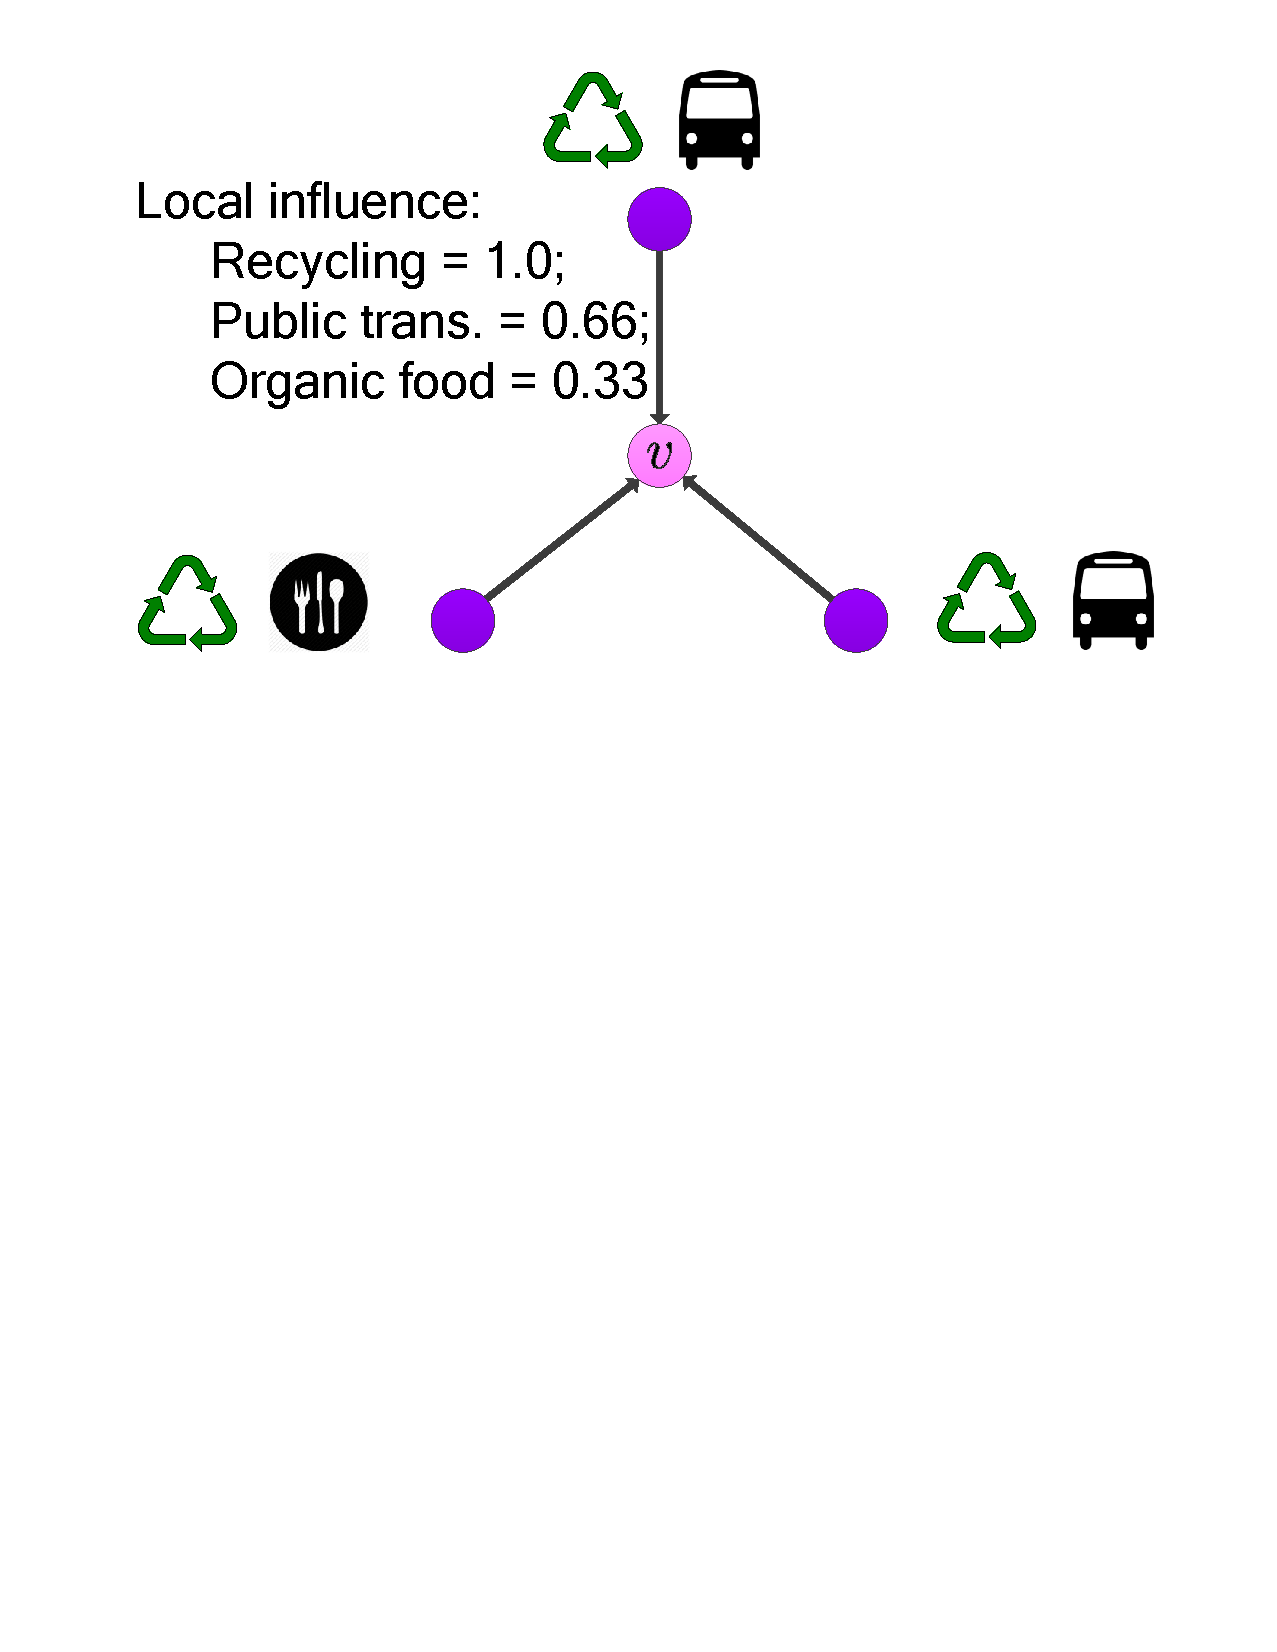
\includegraphics[viewport=1.75in 4in 7in 11in, width=\linewidth]{figs/timeline-2a}}%
\hspace{.2\linewidth}%
\parbox[][][t]{.3\linewidth}{%
\subcaption{The three behaviors and the network.}}
\parbox{.3\linewidth}{
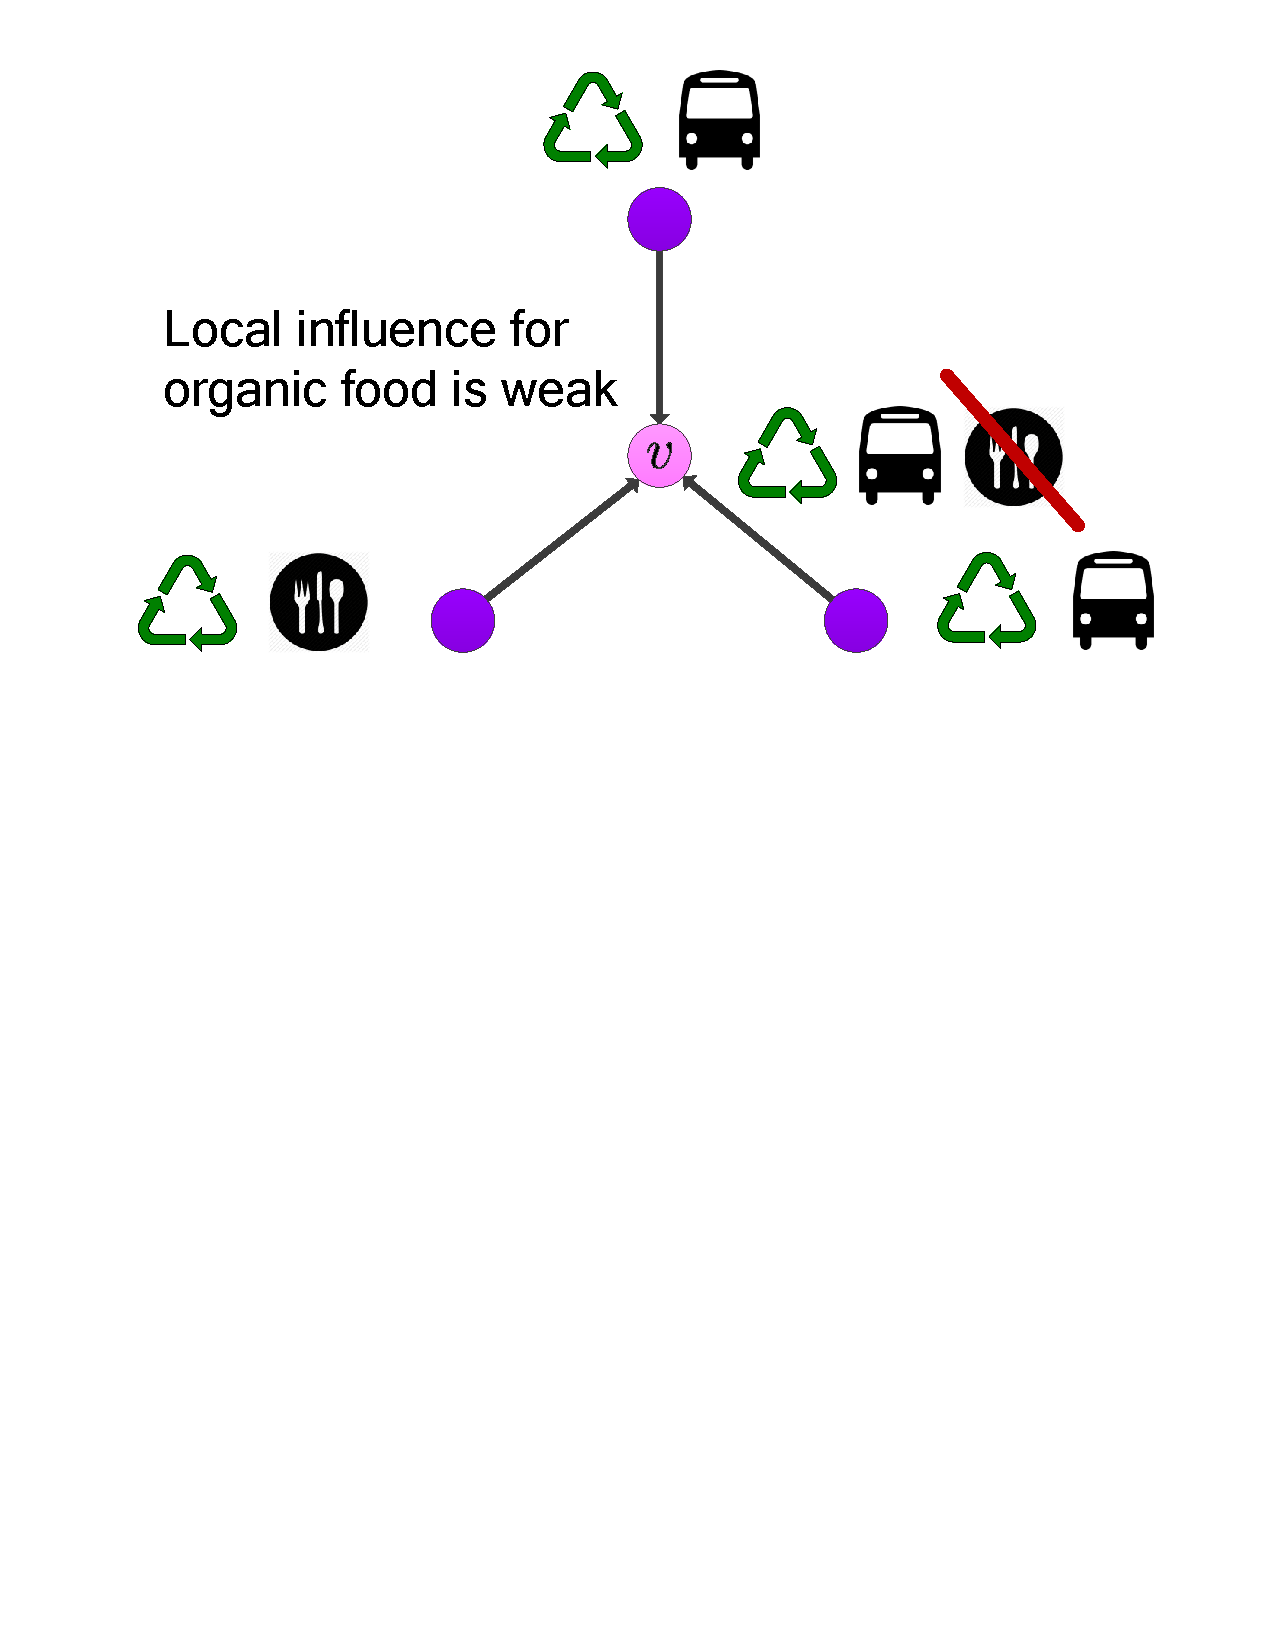
\includegraphics[viewport=1.75in 4in 7in 11in, width=\linewidth]{figs/timeline-3a}}%
\hspace{.2\linewidth}%
\parbox[][][t]{.3\linewidth}{%
\subcaption{The three behaviors and the network.}}
\parbox{.3\linewidth}{
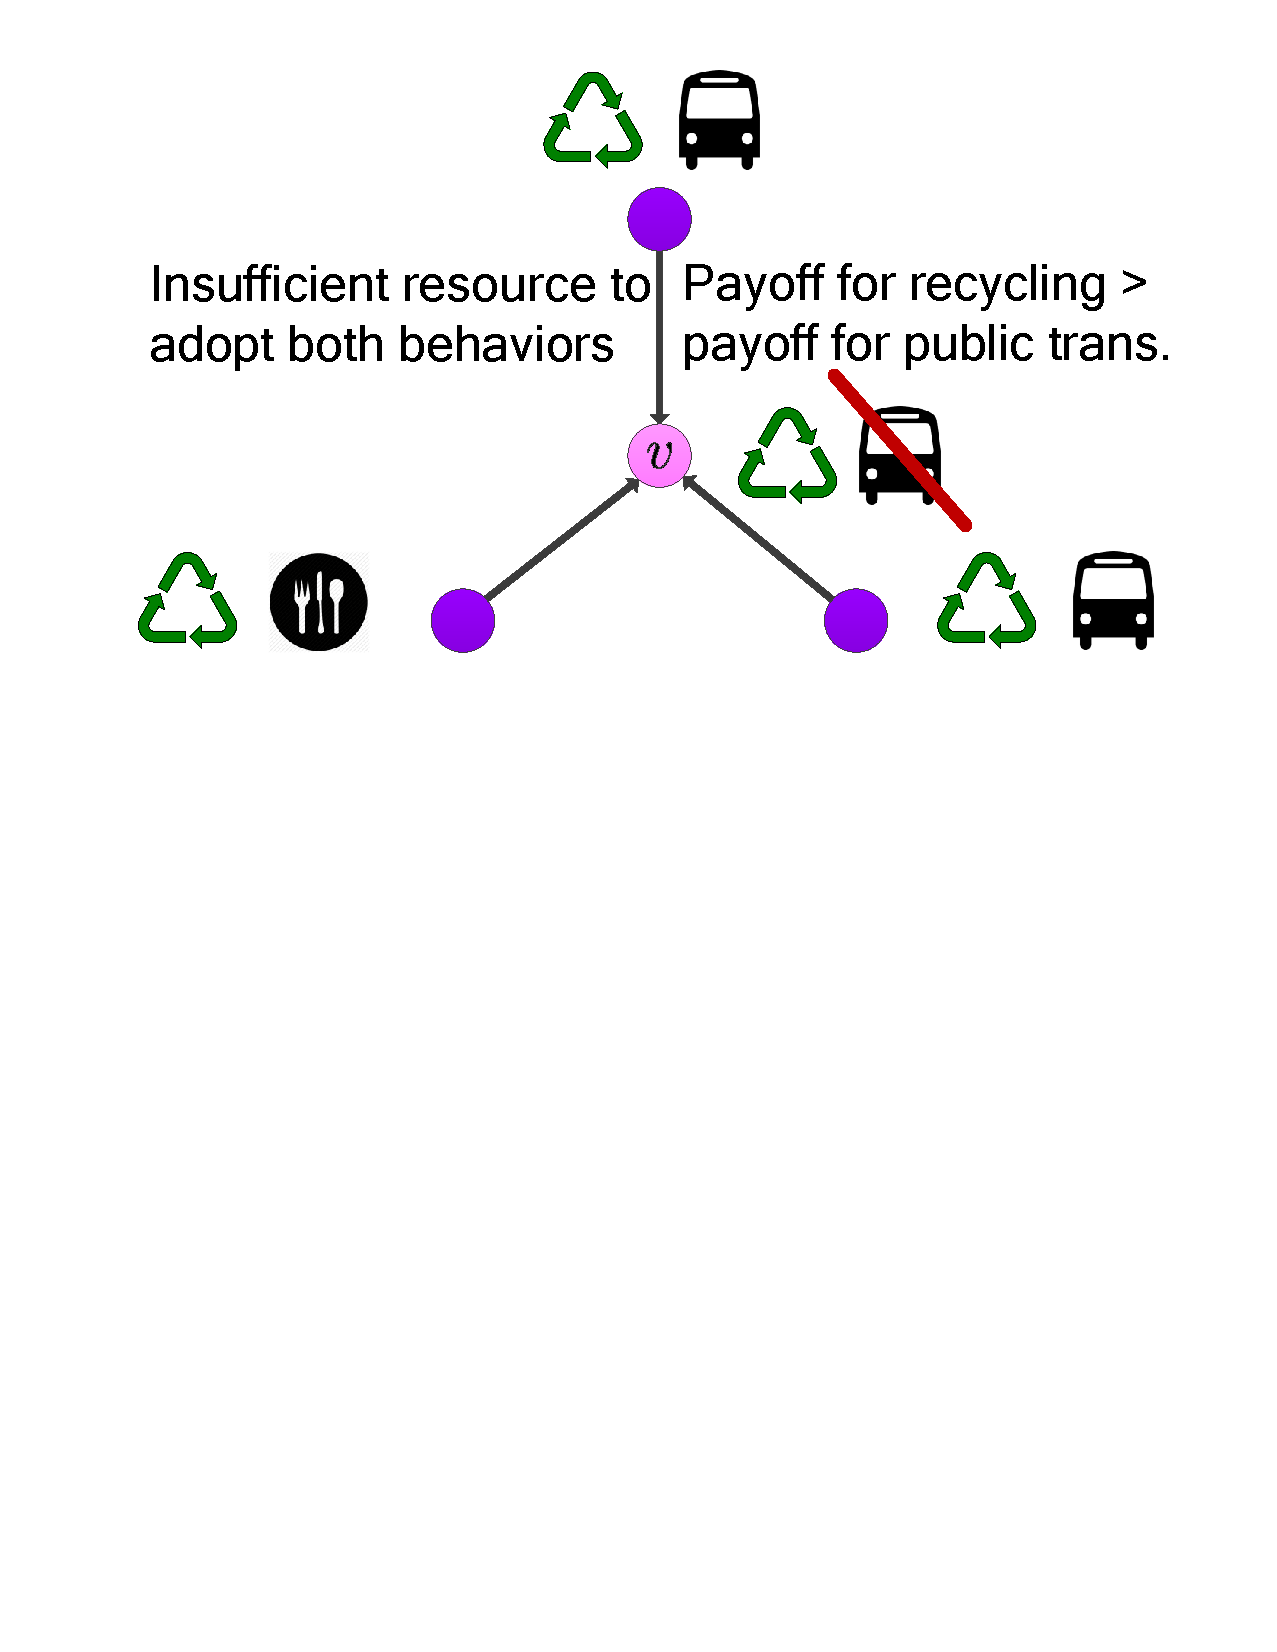
\includegraphics[viewport=1.75in 4in 7in 11in, width=\linewidth]{figs/timeline-4a}}%
\hspace{.2\linewidth}%
\parbox[][][t]{.3\linewidth}{%
\subcaption{The three behaviors and the network.}}
\caption{Multiple behavior adoption model.}
\end{figure}

\begin{figure}[htb]
       		   \begin{subfigure}[b]{0.6\textwidth}
                       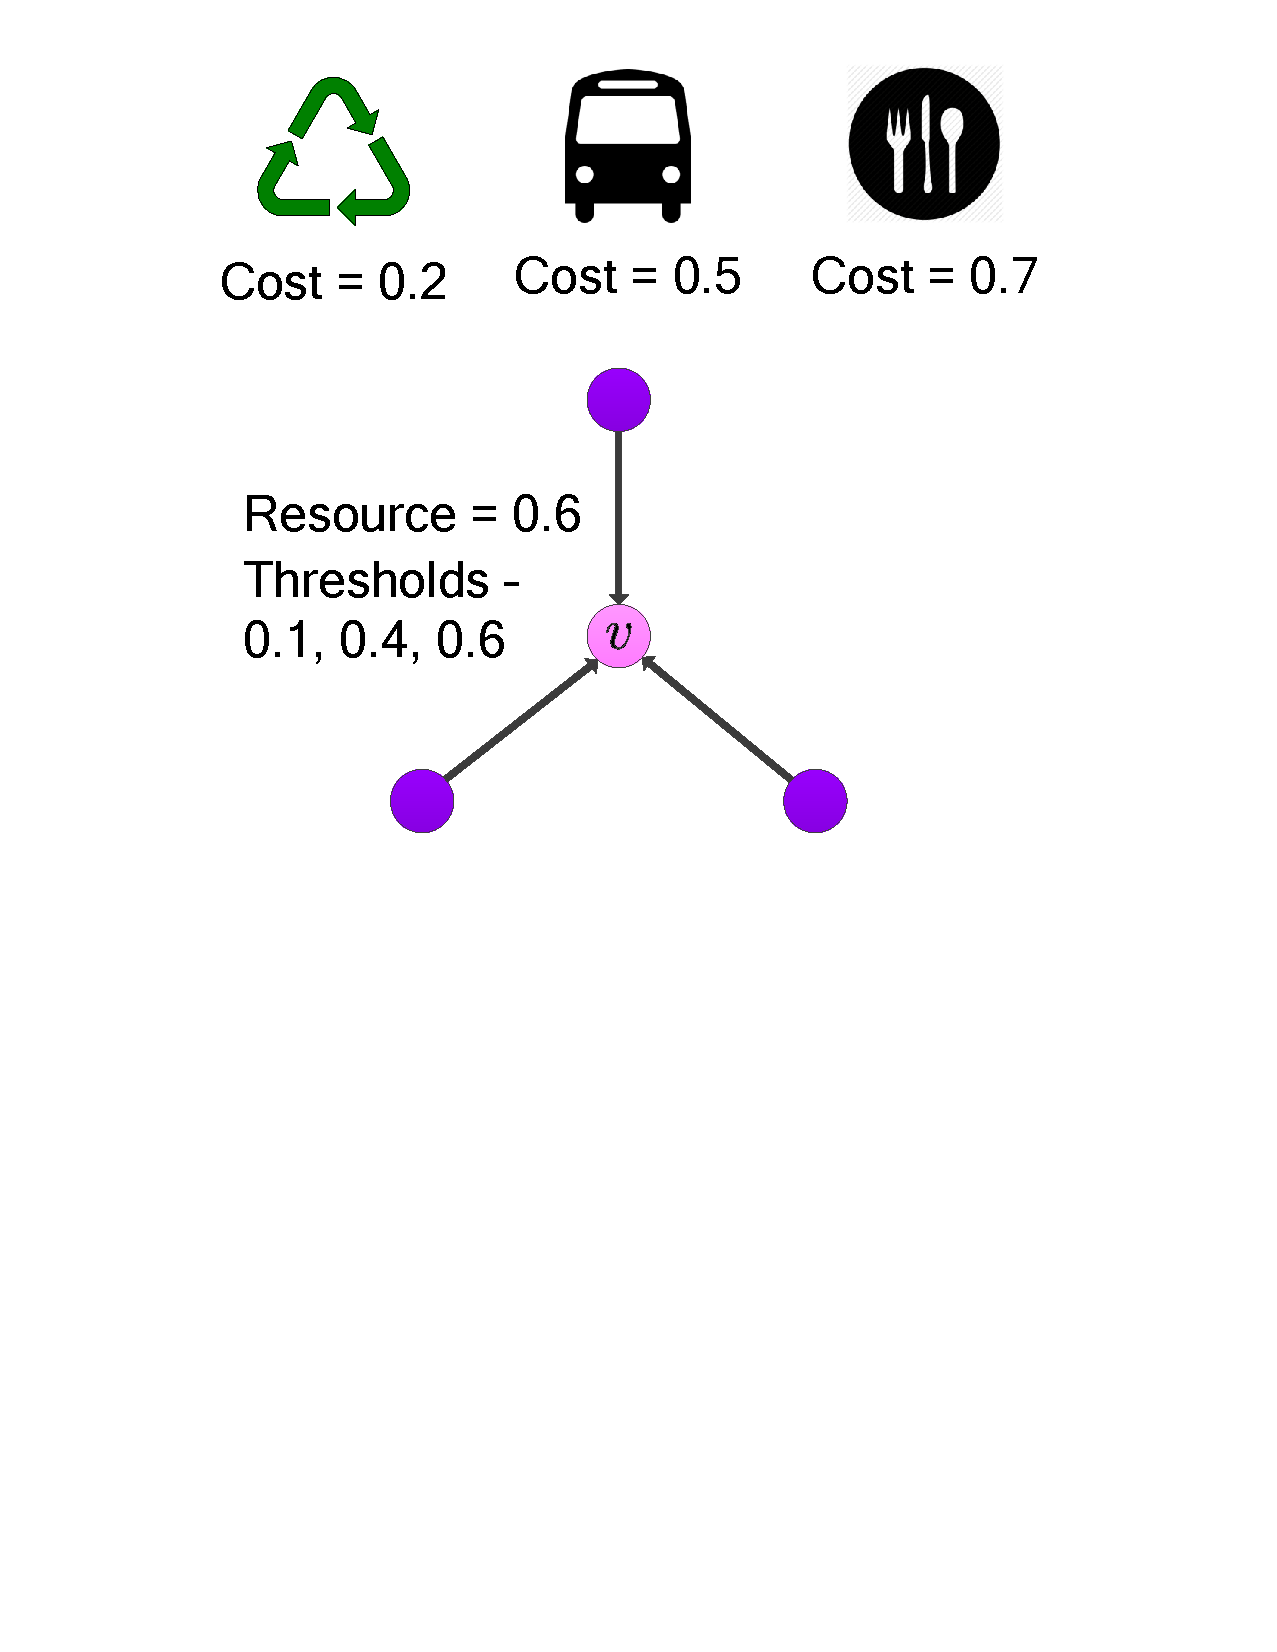
\includegraphics[width=0.6\textwidth]{figs/timeline-1a}
                       \caption{A gull}
                       \label{fig:gull}
               \end{subfigure}
               %~
               
               \begin{subfigure}[b]{0.6\textwidth}
                       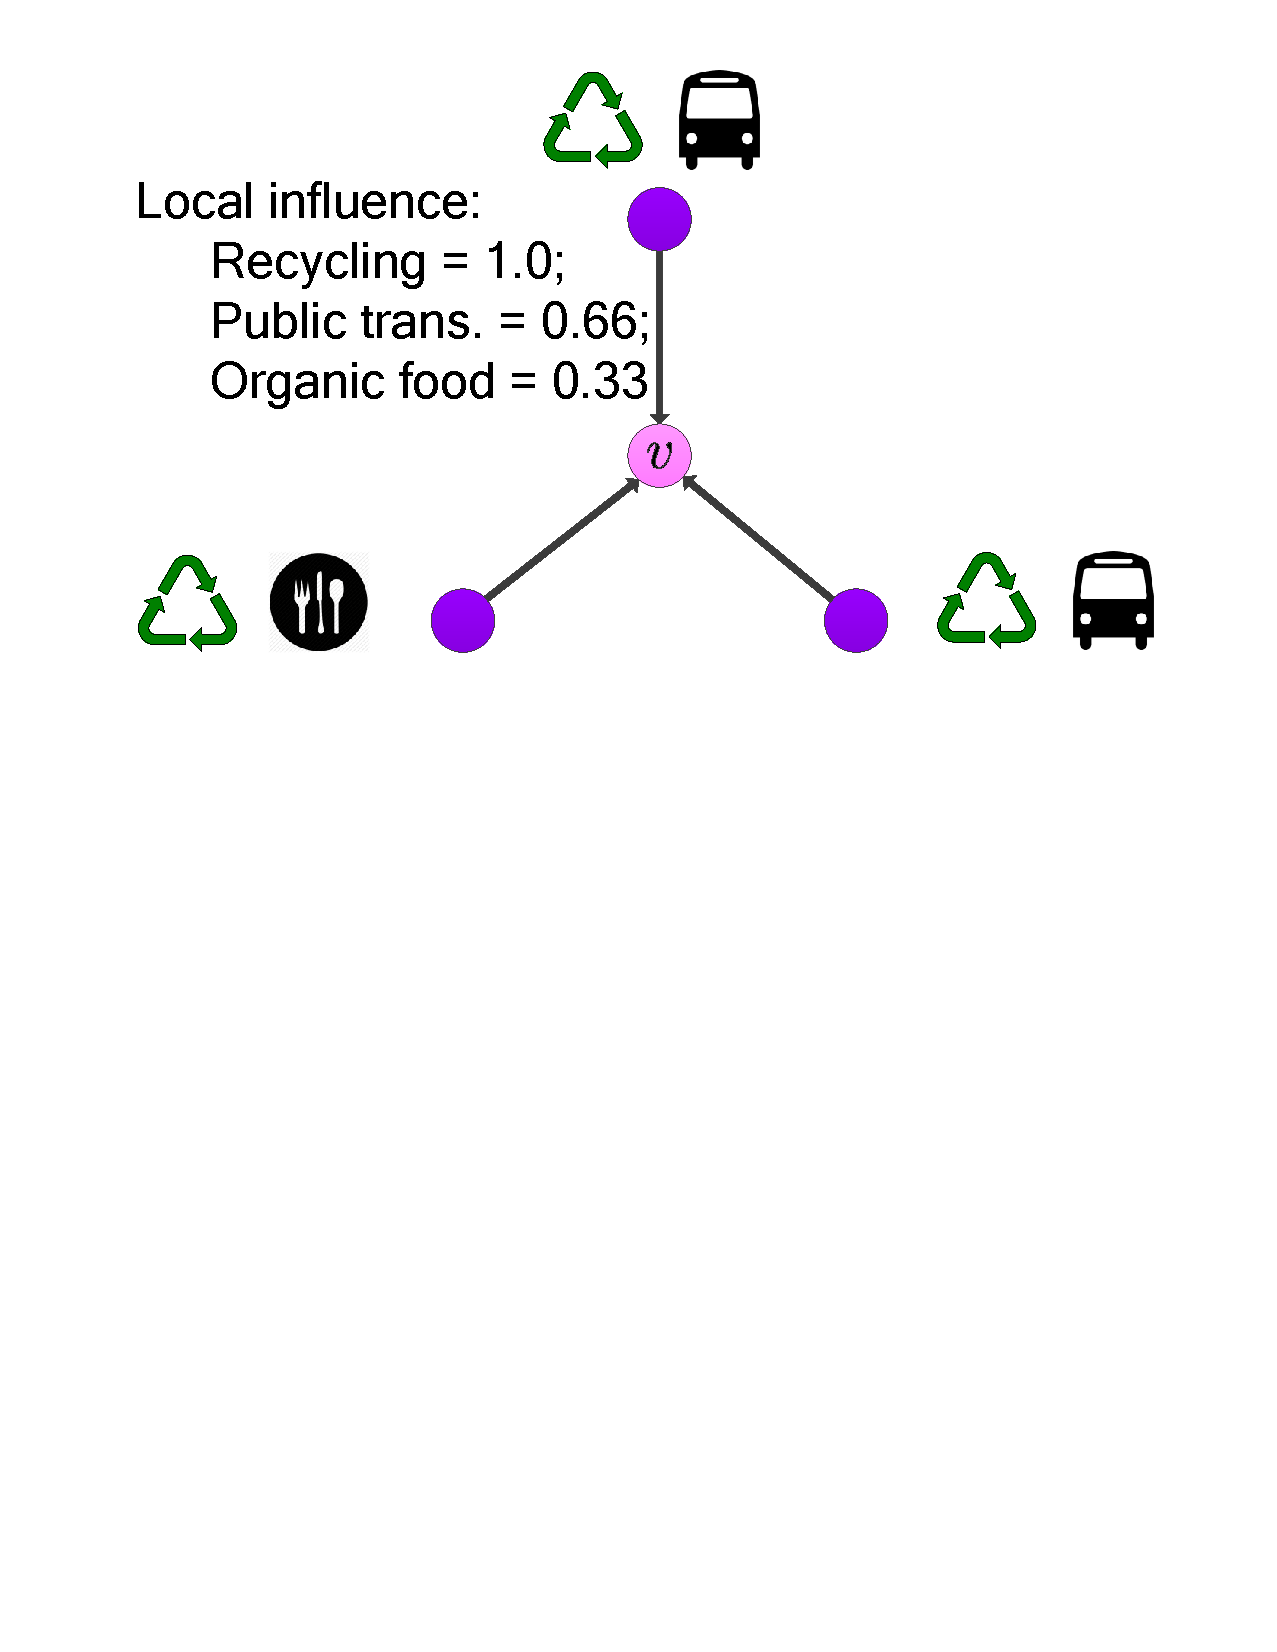
\includegraphics[width=0.6\textwidth]{figs/timeline-2a}
                       \caption{A tiger}
                       \label{fig:tiger}
               \end{subfigure}
               %~
               
               \begin{subfigure}[b]{0.6\textwidth}
                       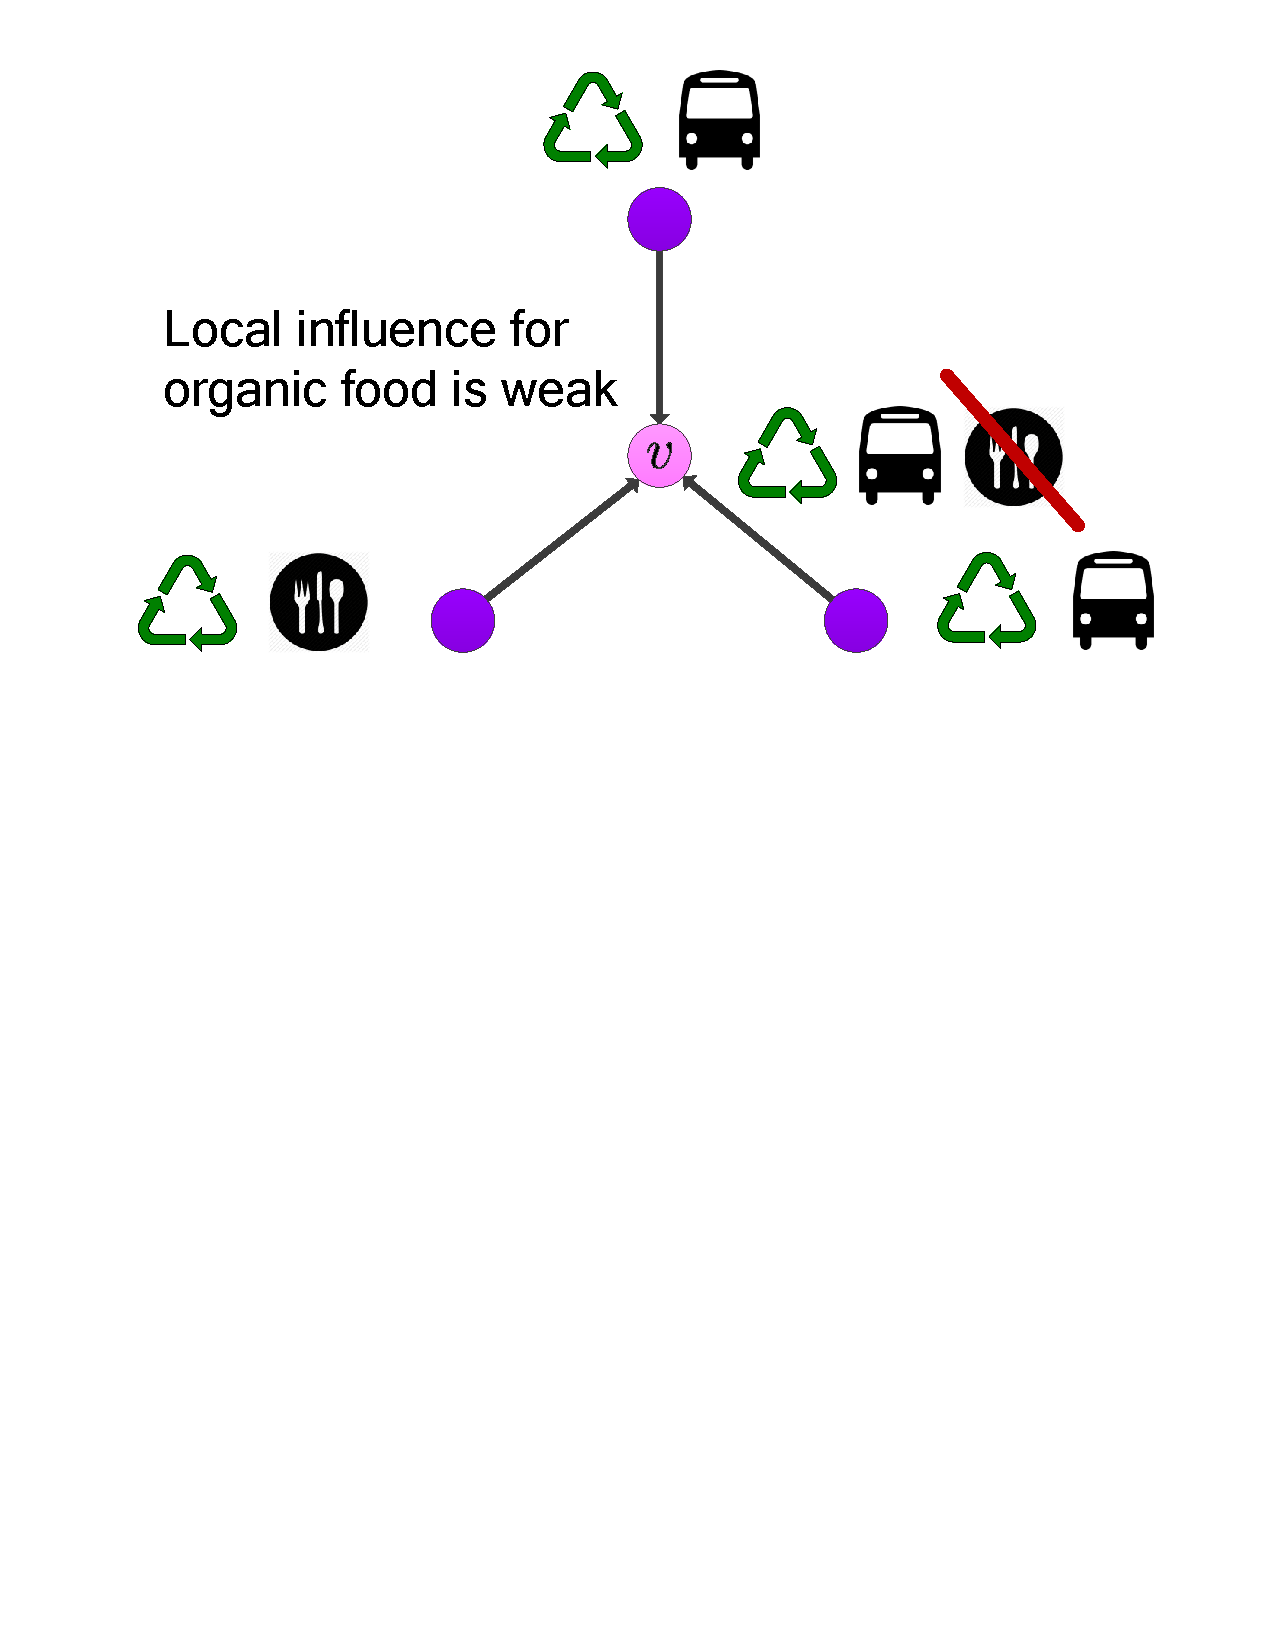
\includegraphics[width=0.6\textwidth]{figs/timeline-3a}
                       \caption{A mouse}
                       \label{fig:mouse}
               \end{subfigure}
               \caption{Pictures of animals}\label{fig:animals}
\end{figure}





\end{document}